\chapter{How does understanding come?}\label{chap:howunder}

Before we talk more about understanding, let us go to the lower level of that first. At the level of perception, we never see the world as it is. Our mind fills up missing information to construct a meaningful seeing. To illustrate the point, let us see Figure \ref{fig:kanizsa}.\footnote{For some more information on Kanizsa triangle, see \url{https://newworldencyclopedia.org/entry/Kanizsa_triangle}.}

\begin{figure}[!hbt]
\centering
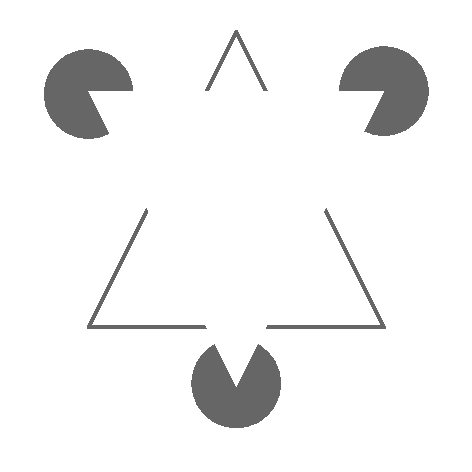
\includegraphics[width=0.6\linewidth]{images/kanizsa}\\
\caption{Kanizsa triangle illusion}
\label{fig:kanizsa}
\end{figure}

In the figure, we cannot help seeing a white triangle floating out of the background and covering a lined triangle and three circles, even though it is not really there. Even the lined triangle and the circles are not really a triangle and full circles. They are just three connected lines and three Pacman shapes arranged in a suggestive way. Some may think the seeing is conditioned by the explanation and its suggestive configuration. Some may insist that they do not really see the hovering triangle. In that case, let us move to Figure \ref{fig:adelson}.\footnote{This checkerboard illusion is published by Edward H.\ Adelson from MIT. For the picture, explanation and proof, see \url{http://persci.mit.edu/gallery/checkershadow}.}

\begin{figure}[!hbt]
\centering
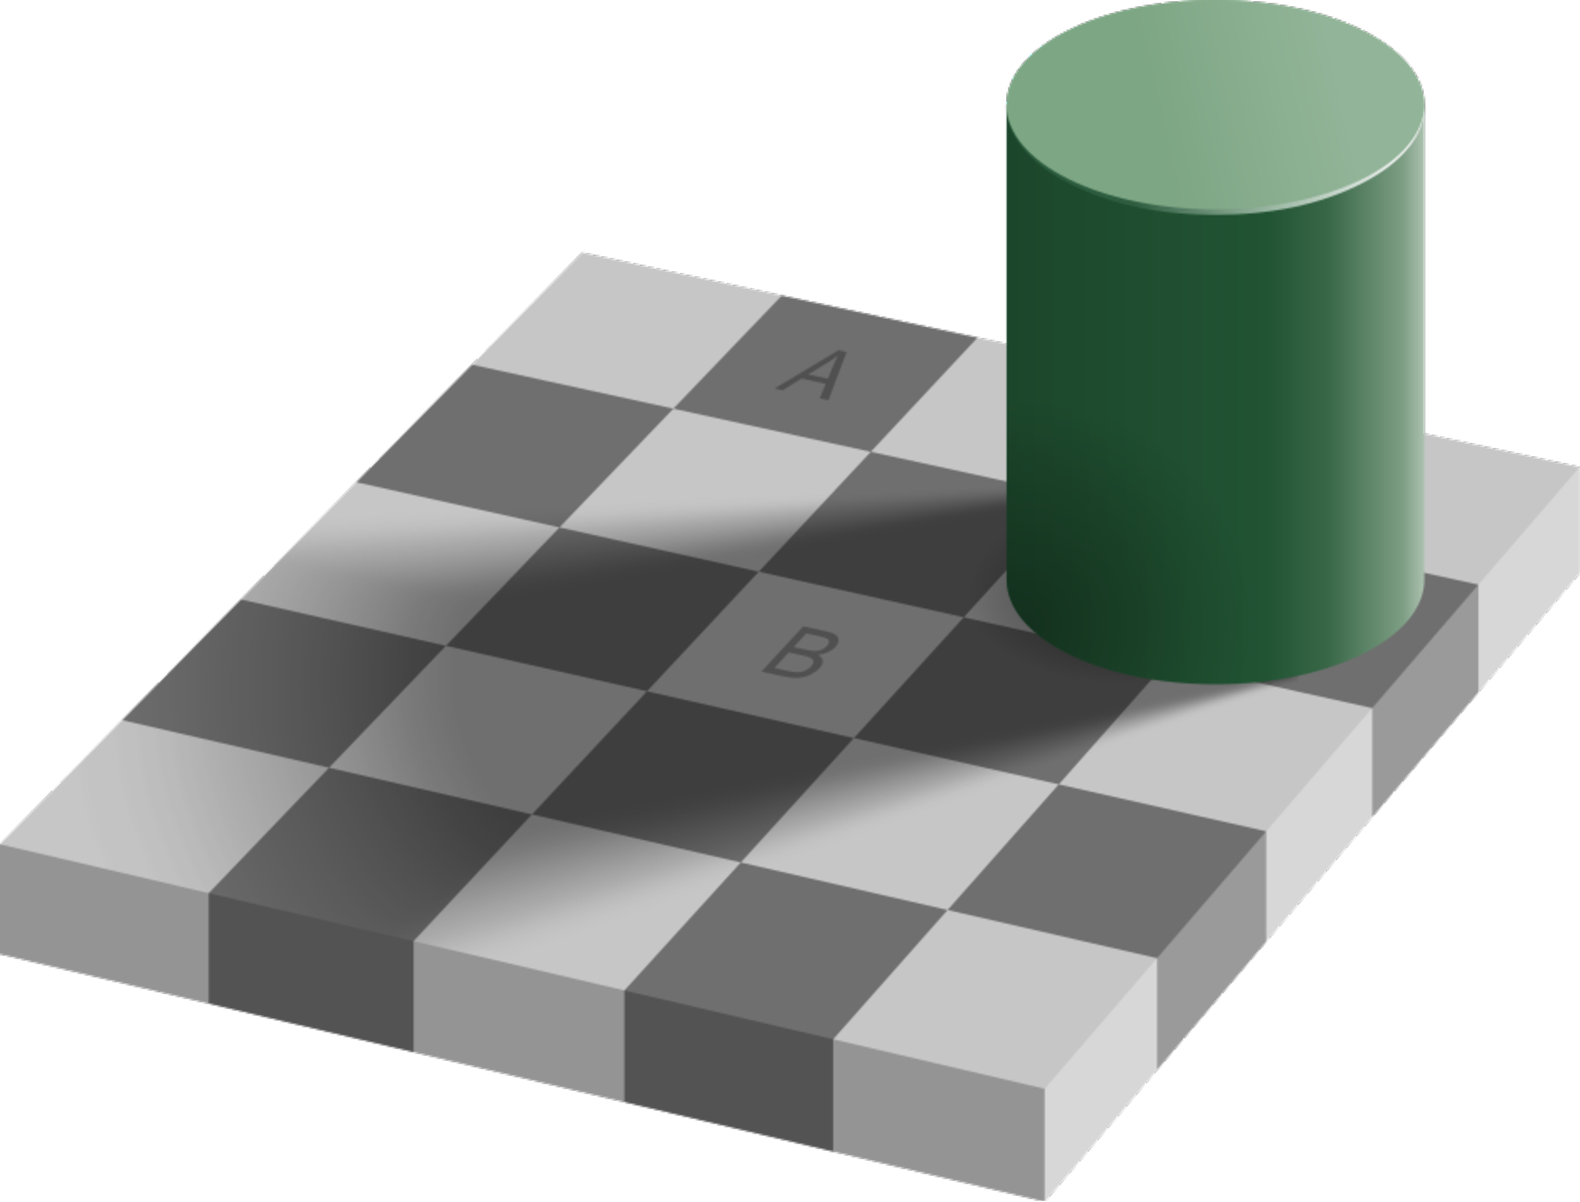
\includegraphics[width=0.8\linewidth]{images/adelson}\\
\caption{Adelson's checkerboard illusion}
\label{fig:adelson}
\end{figure}

In the checkerboard, the squares marked by A and B have the same shade of gray. If you do not believe it, then capture the image, paste it in a paint program, and use eyedropper to test the color. Or easier, go to the website mentioned or search a proof in the Internet. The illusion confirms that we cannot control our seeing. Our brain does some tricks that condition our perception. This constructive nature of perception happens in other senses as well.

Another illustration everyone should know is our visual blind spot. In our eyes, there is an area that has no receptive cells to detect the light, where the optic nerve is connected to the eyeball. So, in principle our visual perception does not produce a complete image, but we see the whole image of the visual field nonetheless, thanks to the filling up by the brain. You can test this blind spot simply by using Figure \ref{fig:blind}.

Here is the instruction: (1) Keep your face at the center of the figure, close one eye and use the other eye stare at the letter in crosswise manner. If you open the right eye, you stare at \textbf{R} on the left side, for example. (2) Slowly move your face towards the image straightly, fixing your eye to the letter. (3) At some point, you will see the other letter you does not fix your eye on disappears. Adjust the position in and out slowly if you do not see as such, keeping your face at the center. The right distance is about three times of the distance between the letters.

From this experiment, you can see that what you see with your eyes is not really what you perceive by your brain. Information from two eyes combines in the way that makes you see the coherent picture of the world. In addition, you can see the 3D world by the combination of two flat images from the two eyes, which are slightly different, thanks to the visual processor in our brain.

\begin{figure}[!hbt]
\centering
\setlength{\unitlength}{1mm}
\begin{picture}(80,20)(0,0)
\put(5,10){\circle{20}}
\put(5,10){\makebox(0,0)[c]{\huge R}}
\put(75,10){\circle{20}}
\put(75,10){\makebox(0,0)[c]{\huge L}}
\end{picture}
\caption{Visual blind spot test}
\label{fig:blind}
\end{figure}

Now let us focus on textual formation process and ponder upon how understanding comes. Philosophically speaking, this is a really big topic. So, I will not go that way. To make things less controversial and well-grounded, I will mostly rely on scientific discourse here.\footnote{The use of `discourse' here is deliberately put. As we shall see later, one discourse does not monopolize the truth. But in my view, scientific discourse or scientific explanation of reality is the most reliable and straight way to see the world. It is less disputable and has strong defensibility.}

Put it simply, understanding is a result of information processing. We get information of the world via our senses. An attempt to make sense of sensory information produces understanding. Once certain understanding is generated and stored, it becomes another information to be used later in the next processing. This means not only external information that is under operation, internal information stored previously (knowledge base)\footnote{I use `knowledge' here in a simple sense---a collection of processed information, or a collection of understanding.} always plays a major role in understanding formation.\footnote{In philosophy, this can be roughly in line with Kantian epistemology. In psychology, this is a Gestalt explanation---``[O]ur perception of the visual world in organized in way that the stimulus input is not \ldots, [therefore] the organization must be contributed by the perceiver'' \citep[p.~61]{reisberg:cognition}.}

To put it another way, our understanding of the world comes from active interplay between the world and the mind. Knowledge structure in our mind is accumulative in nature, and everyone has a unique structure. That means when sensing the same world-data, two persons can have different understanding due to difference in internal knowledge structure formed previously. At the basic level, this difference does not has a significant impact on our living. We can understand each other in conversation. We can read a novel, see a movies and understand the same story line. However, everyone has an experience that sometimes, if not often, our and others' understanding of the same event are not exactly the same.

To conclude, understanding partly comes from external world's information, and partly from our existing knowledge structure. These two parts always work together. Even newly born babies have a kind of bootstrapping knowledge, otherwise they will not survive.\footnote{In biological terms, this is a genetic endowment. Buddhists are tempted to think in terms of previous karma. I think this is quite misleading, because every baby has the same fundamental instinctive responses that are not good or bad but essential to survival. It is a part of our human nature, not a result of particular actions.}
